\documentclass[article.tex]{subfiles}
\begin{document}

\begin{figure}[tb]
\centering
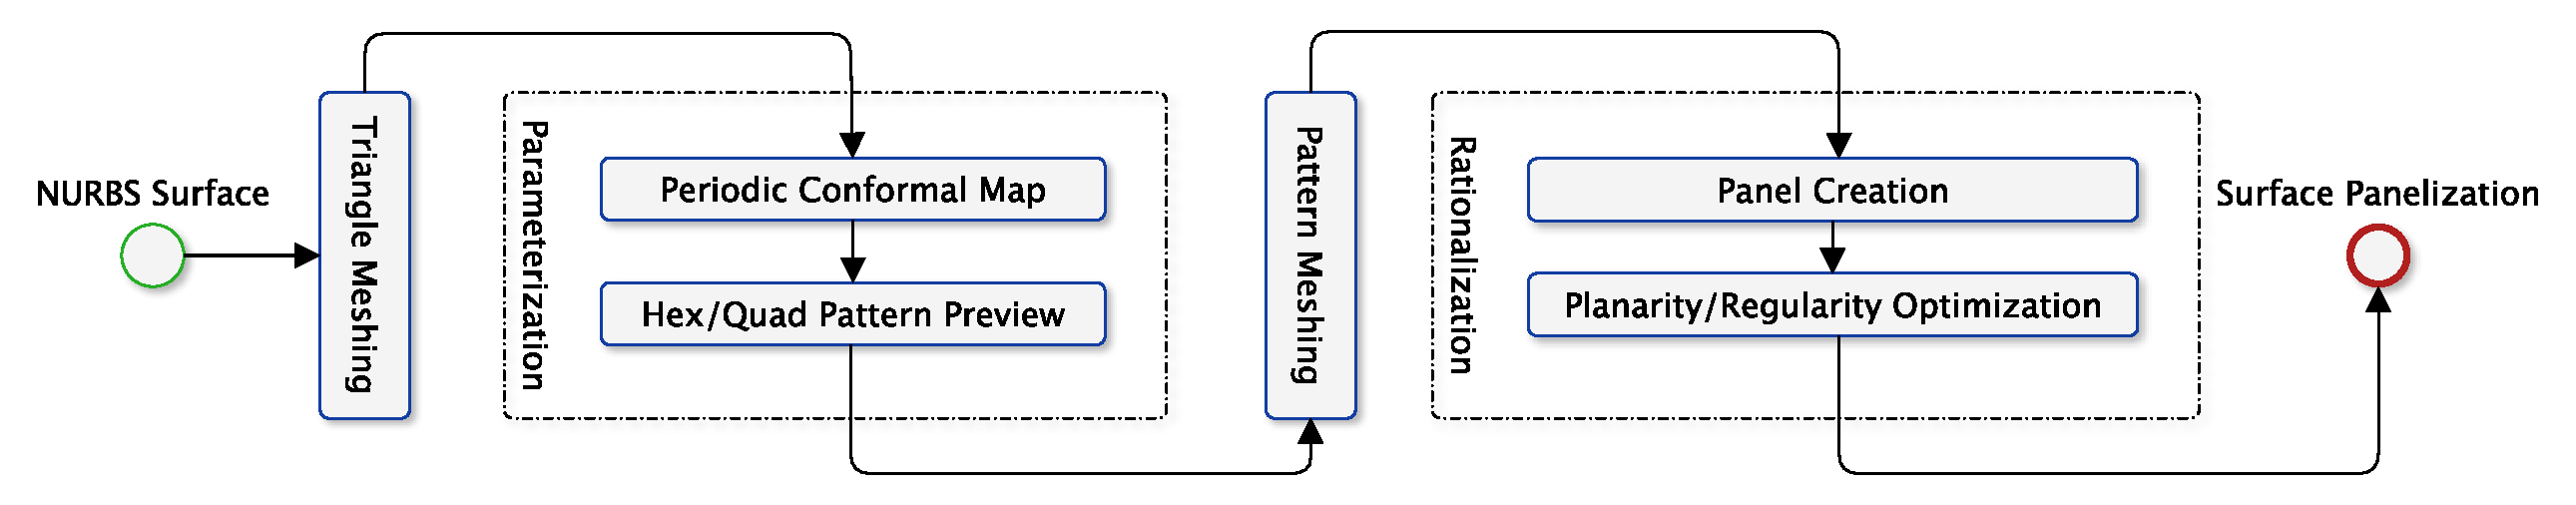
\includegraphics[width=\textwidth]{flowchart_bpmn_horizontal}
\caption{Flow diagram of the algorithms described in this paper. From
  a \nurbs surface a triangle mesh is created. The parameterization
  part is described in Section~\ref{sec:conformal-parameterization}. A
  pattern-mesh is created using this parameterization. The creation
  and optimization of panels is described in
  Section~\ref{sec:regular_hexagons}.}
\label{fig:algorithm_diagram}
\end{figure}

\section{Introduction}
\label{sec:introduction}

The panelization of surfaces remains a challenge in architectural
design. CAD software such as Rhino, delivers powerful \nurbs surface
modelling to the designer. Their ease of use have made them a de facto
standard for the design of freeform (and other) shapes in
architectural design– especially building envelopes and facades.  

The scale of buildings introduces challenges to surface-based
modelling strategies: The large scale of building elements demands
that they are divided into smaller elements. The cost of material and
labor, standardized production lines, green building concepts,
availability and redundancy during construction periods demand for a
high degree of similarity of these elements. Yet, the inherent
UV subdivision of \nurbs surfaces offers limited control over the
layout, shape and configuration of the panels. While strategies for
the controlled and careful creation of freeform surfaces have been
presented (see~\cite{Ceccato}) and realized, the tiling of true
freeform surfaces through alternative algorithms is still a challenge.

The quality of a surface panelization solution can be defined in
various ways. From an aesthetic point of view the shape of individual
elements is important. Further there are global conditions such as
alignment with surface boundaries and smooth transition of element
shape. From the standpoint of fabrication, the elements should be
repetitive. The contributions of this paper are:

\begin{itemize}
\item {\bf Periodic discrete conformal parameterization}:
  % 
  We present an algorithm that maps a triangle mesh with cylinder
  topology conformally to a cylinder or a cone of revolution. This
  allows us to obtain seamless patterns on surfaces. It is a
  generalized version of the discrete conformal parameterization
  scheme described by~\cite{SSP08}.
\item {\bf Regular elements}:
  % 
  We show how the periodic discrete parameterization can be used to
  construct a panelization of the given periodic surface into a small
  number of repeating regular elements.
\item {\bf Applications to architectural design}: 
  % 
  We present a case study that initiated the development and where the
  described methods have successfully been applied in the architectural design
  context.
\end{itemize}

The article is organized as follows:
Section~\ref{sec:parameterization} describes various parameterization
schemes available to architectural geometers. We briefly discuss the
shortcomings of current methods and explain how we adress them with our method.
Section~\ref{sec:conformal-parameterization} introduces the concept of
periodic discrete conformal parameterizations.  See
Figure~\ref{fig:algorithm_diagram} for a schematic view of the
proposed method. In Section~\ref{sec:panelization} we present a case
study that led to the development of this
work. Section~\ref{sec:regular_hexagons} deals with the optimization
of panels to meet requirements arising during the case study. We give
implementational details in Section~\ref{sec:implementation} and close
with an outlook on further research.

\subfilebibliography

\end{document}

%%% Local Variables: 
%%% mode: latex
%%% TeX-master: "article"
%%% End: 
